\documentclass[12pt,a4paper]{article}
\usepackage[utf8]{inputenc}
\usepackage[T1]{fontenc}
\usepackage{graphicx}
\usepackage{geometry}
\geometry{left=3cm,right=2cm,top=3cm,bottom=2cm}
\renewcommand{\baselinestretch}{1.5}
\usepackage{mathptmx}
\usepackage{hyperref}
\hypersetup{colorlinks=true, linkcolor=black, urlcolor=blue}
\begin{document}

% ============ CAPA ============
\begin{titlepage}
\centering
\vspace*{2cm}
{\Large\bfseries UNIVERSIDADE VIRTUAL DO ESTADO DE SÃO PAULO\par}
\vspace{2cm}
{\huge\bfseries Tintas MGMT: Sistema de Organização e\par}
\vspace{0.3cm}
{\large Análise de Dados Empresarial\par}
\vspace{3.5cm}
{\normalsize Jessica Fabiane Costa de Medeiros\par}
{\normalsize Luiz Henrique Ferreira Silva\par}
{\normalsize Mikael Silva\par}
{\normalsize Rafael Massao Okumura\par}
{\normalsize Thainá Alzira Carvalho Vieira Batista\par}
{\normalsize Willian Pires da Silva\par}
\vfill
{\normalsize Araçariguama, Iperó, Itapetininga, Salto - SP\par}
{\normalsize 2026\par}
\end{titlepage}

% ============ RESUMO ============
\pagebreak
\section*{Resumo}

A operação de uma fábrica de tintas envolve diferentes atividades, como compra de matérias-primas, produção, envase, armazenamento, venda de produtos e manutenção de equipamentos. Quando essas informações não são registradas de forma organizada, torna-se difícil acompanhar a quantidade produzida, o volume vendido, os tamanhos de embalagem mais procurados, as cores de maior saída, os níveis de estoque, as perdas e as paradas de máquinas. Essa dificuldade pode prejudicar o planejamento da produção e a tomada de decisões da empresa.

Com base no levantamento inicial realizado junto a uma fábrica de tintas, este trabalho propõe o desenvolvimento do Tintas MGMT, um aplicativo web destinado à organização dos dados operacionais da empresa e à visualização dos resultados. A solução busca reunir informações sobre produção, vendas, estoque, perdas, atrasos e manutenção em uma estrutura única e de fácil consulta. O projeto também está relacionado ao desenvolvimento de análise de dados e à preparação de uma interface para apresentação das informações.

A proposta considera a realidade de uma empresa que trabalha com embalagens de 1 litro, 3,6 litros e 18 litros, possui um tanque de produção de aproximadamente 2.000 litros, motores trituradores, bomba de transferência, tanque para água, envase manual e equipamentos de pintura para locação. O desenvolvimento inicial contempla a definição do problema, o levantamento de requisitos, a criação da estrutura do aplicativo, o cadastro das informações básicas e a elaboração dos wireframes das principais telas. A continuidade do projeto deverá permitir a substituição de registros dispersos por dados organizados, possibilitando análises mais precisas e melhorias no acompanhamento da operação.

\textbf{Palavras-chave:} Aplicativo web; análise de dados; fábrica de tintas; produção; estoque; manutenção; visualização de informações.
\pagebreak

% ============ SUMÁRIO ============
\tableofcontents
\pagebreak

% ============ LISTA DE FIGURAS ============
\listoffigures
\pagebreak

% ============ LISTA DE ILUSTRAÇÕES ============
\section*{Lista de Ilustrações}
\pagebreak

% ============ CORPO ============
\section{Introdução}
A escolha deste tema surgiu a partir do contato com uma empresa do segmento de fabricação de tintas e do levantamento inicial de suas atividades. A empresa trabalha com a fabricação e o envase de tintas em diferentes tamanhos de embalagem, realiza compras de fornecedores, mantém estoque de matérias-primas e produtos acabados e realiza revisões periódicas em seus equipamentos. Também possui máquinas de pintura destinadas à locação.

Durante as conversas iniciais, foram identificados alguns dos principais elementos da operação: um tanque de tinta com capacidade aproximada de 2.000 litros, três motores trituradores, uma bomba responsável pelo deslocamento da tinta, um tanque para água e um equipamento de envase manual. A empresa trabalha com embalagens de 1 litro, 3,6 litros e 18 litros e informou uma produção média aproximada de 150 baldes por semana.

Essas informações mostram que existe uma operação produtiva que pode ser acompanhada por meio de dados. Entretanto, conhecer apenas a quantidade aproximada produzida não é suficiente para compreender o desempenho da fábrica. É necessário saber quais produtos foram fabricados, quais cores foram utilizadas, quais tamanhos de embalagem foram produzidos, quanto foi vendido, quais matérias-primas foram consumidas e quais equipamentos permaneceram parados.

A ausência de registros organizados pode dificultar o planejamento e fazer com que decisões importantes sejam tomadas com base apenas na memória ou em anotações separadas. Também pode dificultar a identificação de perdas e atrasos. Uma parada em um motor, uma falha na bomba ou uma revisão não realizada podem interferir na produção e no cumprimento dos prazos de entrega.

Nesse contexto, o presente trabalho concentra-se na concepção e no desenvolvimento inicial do Tintas MGMT, um aplicativo web voltado à organização dos dados de uma fábrica de tintas. A proposta é reunir informações relevantes da operação e apresentar os resultados de forma simples, permitindo que a empresa acompanhe sua produção, vendas, estoque e manutenção com maior clareza.

O projeto também se relaciona ao tema de desenvolvimento de análise de dados em escala utilizando conjuntos de dados existentes ou capturados por dispositivos e aprendizagem de máquina, preparando uma interface para visualização dos resultados. Nesta etapa, o foco está na organização da base de informações e na definição da interface. A utilização de dados históricos, sensores e modelos de análise deverá ocorrer conforme a aplicação evolua e conforme a empresa disponha de registros suficientes.

\section{Desenvolvimento}

\subsection{Objetivos}
\subsubsection*{Objetivo geral}
Desenvolver um aplicativo web capaz de organizar dados de produção, vendas, estoque, perdas, atrasos e manutenção de uma fábrica de tintas, permitindo visualizar as principais informações da operação e apoiando o planejamento da empresa.

\subsubsection*{Objetivos específicos}
\begin{itemize}
\item Identificar as principais atividades realizadas pela fábrica de tintas.
\item Levantar as informações necessárias para acompanhar a produção, o envase, as vendas e o estoque.
\item Registrar produtos, cores, embalagens, matérias-primas, fornecedores e equipamentos.
\item Organizar informações referentes aos lotes produzidos e às quantidades planejadas e realizadas.
\item Acompanhar a saída de produtos por tamanho de embalagem e por cor.
\item Controlar a entrada e a saída de matérias-primas e produtos acabados.
\item Registrar perdas, atrasos e possíveis causas relacionadas à produção.
\item Organizar as revisões e as paradas dos equipamentos utilizados pela empresa.
\item Criar uma interface simples para apresentação dos indicadores e resultados.
\item Preparar uma base de dados que possa ser utilizada em análises posteriores.
\item Avaliar o protótipo inicial e propor melhorias para a continuidade do projeto.
\end{itemize}

\subsection{Justificativa e delimitação do problema}
A fabricação de tintas depende da disponibilidade de materiais, equipamentos, mão de obra, embalagens e espaço para armazenamento. Uma falha em qualquer uma dessas etapas pode interferir na produção. Além disso, os produtos podem possuir diferentes cores, volumes e destinos, o que aumenta a necessidade de organizar os registros.

A informação de que a empresa produz aproximadamente 150 baldes por semana representa apenas uma visão geral. Para apoiar decisões, é necessário detalhar essa produção. Deve-se identificar quantos baldes correspondem às embalagens de 1 litro, 3,6 litros e 18 litros, quais cores são mais requisitadas, quais produtos permanecem em estoque e quais itens precisam ser repostos.

A mesma necessidade existe em relação às vendas. Saber o total vendido é importante, mas também é necessário observar o comportamento da demanda. Uma determinada embalagem pode possuir maior saída em um período, enquanto uma cor pode ser mais procurada em determinada época. A organização desses dados pode ajudar a empresa a planejar melhor suas compras e sua produção.

A manutenção também precisa ser considerada. A empresa realiza revisões periódicas, e os equipamentos possuem relação direta com a continuidade da produção. Registrar a data de uma revisão, o equipamento envolvido, o tipo de manutenção e o tempo de parada pode ajudar a compreender a origem de atrasos e perdas.

A justificativa social e econômica deste projeto está relacionada à possibilidade de apoiar uma empresa real na organização de suas atividades. Um sistema simples e centralizado pode facilitar a consulta de informações, reduzir a dependência de registros dispersos e contribuir para decisões mais seguras. A solução também pode apoiar o crescimento da empresa, pois uma base organizada facilita a identificação de necessidades e oportunidades.

A justificativa acadêmica está relacionada à aplicação de conhecimentos de desenvolvimento web, banco de dados, organização da informação, análise de dados e visualização. O trabalho permite estudar um problema real e transformá-lo em uma proposta tecnológica, passando pelas etapas de levantamento, definição de requisitos, modelagem, construção de protótipo e avaliação inicial.

Diante dessas necessidades, formula-se a seguinte pergunta-problema que orienta este estudo: Como desenvolver uma solução digital simples e organizada capaz de reunir os dados de produção, vendas, estoque, perdas e manutenção de uma fábrica de tintas, facilitando o acompanhamento da operação e a visualização dos resultados?

A delimitação do problema concentra-se no desenvolvimento inicial de um aplicativo web para uso interno da empresa. O protótipo contempla a estrutura de acesso, os cadastros básicos, a organização das áreas do sistema e a definição das principais telas. Nesta etapa, os módulos de produção, pedidos, estoque, perdas, manutenção e relatórios ainda não estão completamente finalizados. Também não fazem parte do escopo inicial a automação direta das máquinas, a emissão fiscal, a integração contábil ou a implantação imediata de sensores.

\subsection{Fundamentação teórica}
A análise de dados tem sido utilizada pelas organizações para transformar registros do cotidiano em informações que apoiem decisões. Em uma indústria, esses registros podem estar relacionados à quantidade produzida, ao consumo de materiais, às vendas, aos estoques, às perdas e ao funcionamento dos equipamentos. Quando as informações são organizadas, torna-se possível observar comportamentos, comparar períodos e identificar situações que precisam de atenção.

No contexto de uma fábrica de tintas, a análise de dados pode contribuir para acompanhar a produção e relacioná-la com a demanda. O histórico de vendas pode indicar quais produtos, cores e embalagens são mais procurados. O histórico de estoque pode demonstrar quais matérias-primas precisam ser repostas com maior frequência. O registro de perdas pode indicar em quais etapas do processo ocorrem maiores desvios.

A análise também pode ser utilizada no acompanhamento da manutenção. Os equipamentos da fábrica possuem influência direta na produção, e as paradas podem causar atrasos. Ao registrar revisões, falhas e períodos de indisponibilidade, a empresa pode compreender melhor o comportamento de suas máquinas e planejar suas atividades de maneira preventiva.

O conceito de Indústria 4.0 está associado à utilização de tecnologias digitais para ampliar a integração e o acompanhamento dos processos industriais. Nesse cenário, os dados podem ser obtidos por registros realizados pelos funcionários ou por dispositivos instalados nas máquinas. Sensores de temperatura, vibração, corrente elétrica ou tempo de funcionamento poderiam, em uma etapa futura, complementar as informações cadastradas no sistema.

A aprendizagem de máquina também pode ser utilizada em projetos de análise industrial, desde que exista uma quantidade adequada de dados históricos. Com registros organizados, poderiam ser estudadas possibilidades como previsão de demanda, identificação de comportamentos fora do padrão e avaliação de risco de paradas. No entanto, a construção de modelos não deve acontecer antes da definição correta dos dados e da verificação da qualidade dos registros.

A interface de visualização é importante porque permite apresentar as informações de maneira mais acessível. Indicadores, tabelas e gráficos podem auxiliar a gestão a compreender os dados sem precisar consultar diretamente registros técnicos. Uma tela de produção pode mostrar os lotes e seus status. Uma tela de estoque pode mostrar os saldos e os itens abaixo do mínimo. Uma tela de manutenção pode apresentar revisões pendentes e equipamentos parados.

A organização das informações deve considerar os princípios de usabilidade e design centrado no usuário. Norman (2013) afirma que os produtos devem ser desenvolvidos considerando as necessidades e limitações das pessoas que irão utilizá-los. Nielsen (1994) também destaca a importância da simplicidade, da clareza e da facilidade de aprendizagem nos sistemas interativos. Esses princípios são relevantes para uma aplicação que será utilizada por pessoas com diferentes níveis de familiaridade com ferramentas digitais.

A modelagem de dados representa outra parte importante da solução. De acordo com Elmasri e Navathe (2019), bancos relacionais podem contribuir para a organização, a consistência e a integridade das informações. No projeto, produtos, cores, embalagens, materiais, equipamentos e fornecedores devem possuir relações organizadas, evitando repetição e facilitando a consulta dos dados.

O desenvolvimento de aplicações web também exige atenção à segurança. O OWASP Top 10 destaca riscos relacionados à autenticação, ao controle de acesso e à exposição inadequada de informações. Por esse motivo, o aplicativo foi planejado com acesso por usuário, perfis de utilização e restrições para as áreas internas do sistema.

Dessa forma, o Tintas MGMT reúne conceitos de análise de dados, organização da informação, usabilidade, banco de dados e desenvolvimento web. A aplicação desses conhecimentos busca criar uma solução simples e adequada ao problema identificado, sem perder a possibilidade de evolução para análises mais avançadas no futuro.

\subsection{Metodologia}
A metodologia utilizada possui caráter de pesquisa aplicada, pois procura desenvolver uma solução para um problema identificado em uma empresa real. Também apresenta caráter exploratório, uma vez que o processo da fábrica ainda está sendo detalhado, e descritivo, porque busca representar as principais atividades, equipamentos e informações envolvidas na operação.

A primeira etapa foi o levantamento inicial do problema. Foram identificados os equipamentos utilizados na produção, os tamanhos de embalagem, a produção aproximada por semana, a existência de estoque de matérias-primas e produtos acabados, as revisões periódicas e a necessidade de acompanhar vendas, perdas e atrasos.

A segunda etapa foi a definição dos requisitos. Foram consideradas as informações de produtos, cores, embalagens, fornecedores, materiais, equipamentos, tanques, clientes, pedidos, lotes, movimentações de estoque, perdas, manutenções e paradas. Também foram definidos os usuários que poderão utilizar o sistema, como administração, gestão, produção, estoque, vendas e manutenção.

A terceira etapa foi a organização da estrutura inicial do aplicativo. Foi desenvolvido um aplicativo web com telas de autenticação, painel principal, cadastros e áreas reservadas para produção, pedidos, estoque, compras, perdas, manutenção e relatórios. A solução utiliza tecnologias web modernas e um banco de dados para armazenar as informações, mas esses detalhes são considerados parte da implementação e não alteram a finalidade principal do projeto.

A quarta etapa foi a criação da estrutura inicial do banco de dados. Foram previstos cadastros para unidades de medida, cores, embalagens, produtos, clientes, fornecedores, materiais, equipamentos, tanques e motivos de perda e atraso. Também foram definidos perfis de acesso para controlar as áreas que cada usuário poderá consultar ou alterar.

A quinta etapa foi a elaboração dos wireframes. Os wireframes foram construídos como rascunhos de baixa fidelidade, utilizando contornos simples, campos, tabelas e áreas reservadas. O objetivo foi representar a organização das telas antes da definição do visual final. Foram planejadas telas para dashboard, produção, estoque e manutenção.

A sexta etapa foi a avaliação preliminar do protótipo. A estrutura de acesso, os perfis e os cadastros iniciais já foram desenvolvidos. O dashboard possui informações demonstrativas para validar a disposição dos elementos, enquanto os módulos operacionais ainda deverão receber os registros reais da empresa.

A continuidade do trabalho deverá incluir a criação dos registros de produção, pedidos, estoque, perdas e manutenção. Depois disso, deverão ser definidos os indicadores que serão apresentados na interface. A validação deverá ocorrer com a comparação entre os registros do sistema e as informações utilizadas pela empresa, verificando se as telas são compreensíveis e se os resultados correspondem à realidade da operação.

\subsection{Resultados preliminares: solução inicial}
Os resultados preliminares obtidos até o momento refletem o avanço na compreensão do problema e na organização da solução proposta para a fábrica de tintas. O levantamento inicial permitiu identificar os principais equipamentos, os tamanhos de embalagem, a produção aproximada e as áreas que precisam ser acompanhadas.

Com base nos requisitos levantados, iniciou-se a elaboração do Tintas MGMT, contemplando telas de acesso, painel principal, cadastros e áreas destinadas à produção, aos pedidos, ao estoque, às perdas e à manutenção. A aplicação foi organizada para permitir a evolução gradual do projeto, começando pelas informações básicas e avançando posteriormente para os registros operacionais.

A estrutura inicial já contempla o cadastro de produtos, cores, embalagens, clientes, fornecedores, materiais, equipamentos e tanques. Também foram definidos perfis de usuário, permitindo que as áreas do sistema sejam relacionadas às responsabilidades de cada pessoa. Essa organização representa uma etapa importante, pois evita que os dados sejam inseridos sem padrão e facilita a construção dos indicadores.

O dashboard foi planejado para apresentar uma visão geral da operação, com informações sobre produção, vendas, estoque e manutenção. Nesta etapa, os dados apresentados são demonstrativos e servem para avaliar a organização da interface. Eles não representam resultados reais da empresa. A substituição por dados reais deverá ocorrer depois da implementação das tabelas de produção, vendas, estoque e manutenção.

As principais dificuldades encontradas estão relacionadas à transformação de uma descrição inicial da operação em informações que possam ser registradas pelo sistema. A produção aproximada de 150 baldes por semana precisa ser detalhada por embalagem, cor, produto e período. Também é necessário definir o momento em que o produto acabado entra no estoque e como os consumos e perdas serão registrados.

Outra dificuldade está relacionada ao acompanhamento das máquinas. A empresa realiza revisões periódicas, mas ainda é necessário registrar com maior precisão os equipamentos envolvidos, os tipos de manutenção, o período de parada e a relação entre a manutenção e os atrasos na produção. Essas definições serão importantes para que os indicadores representem o funcionamento real da fábrica.

Os wireframes apresentados nos anexos representam a primeira organização das telas. Eles foram feitos de maneira simples, como rascunhos, para demonstrar os campos e informações necessários. A tela de dashboard apresenta indicadores gerais. A tela de produção apresenta lotes e quantidades. A tela de estoque apresenta itens e saldos. A tela de manutenção apresenta equipamentos, revisões e paradas.

De modo geral, os resultados preliminares confirmam a pertinência da proposta. O Tintas MGMT possui uma estrutura inicial capaz de receber os dados da empresa e transformá-los em informações organizadas. O protótipo desenvolvido representa um primeiro passo para a criação de uma solução de acompanhamento operacional e estabelece a base para os ajustes que serão realizados na continuidade do projeto.

\section{Referências}
ABNT – Associação Brasileira de Normas Técnicas. NBR 14724: Informação e documentação – Trabalhos acadêmicos – Apresentação. Rio de Janeiro: ABNT, 2011.

ELMASRI, Ramez; NAVATHE, Shamkant. Sistemas de Banco de Dados. 7. ed. São Paulo: Pearson, 2019.

IBM. Cross-Industry Standard Process for Data Mining – CRISP-DM. Disponível em: https://www.ibm.com/docs/en/spss-modeler/cross-industry-standard-process-for-data-mining. Acesso em: 2026.

NIELSEN, Jakob. Usability Engineering. Cambridge: Academic Press, 1994.

NORMAN, Donald. The Design of Everyday Things. Revised and expanded edition. New York: Basic Books, 2013.

OWASP. OWASP Top 10. Disponível em: https://owasp.org/Top10/. Acesso em: 2026.

REACT. React Learn. Disponível em: https://react.dev/learn. Acesso em: 2026.

SUPABASE. Local Development and Row Level Security Documentation. Disponível em: https://supabase.com/docs/. Acesso em: 2026.

TANSTACK. TanStack Router Documentation. Disponível em: https://tanstack.com/router/latest/docs/framework/react/overview. Acesso em: 2026.

\section{Anexos}
\begin{figure}[h]
\centering
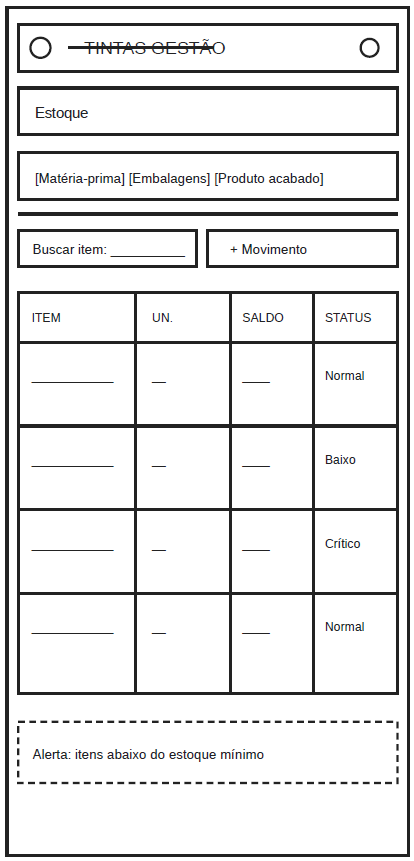
\includegraphics[width=0.45\textwidth]{figures/img1.png}
\caption{Wireframe Gestão}
\label{fig:gestao}
\end{figure}

\begin{figure}[h]
\centering
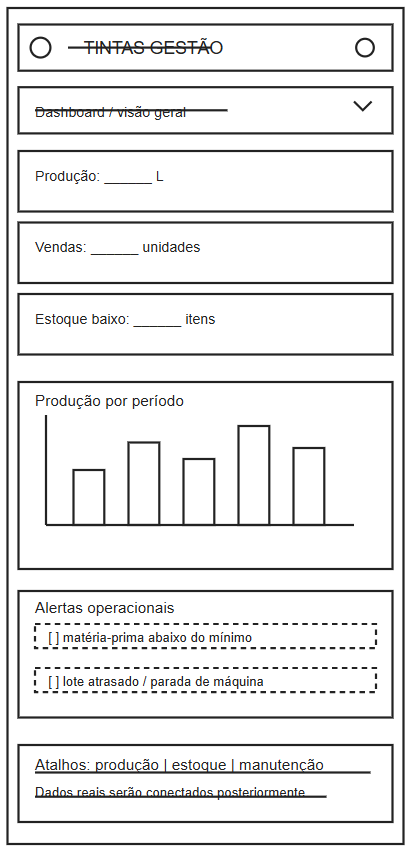
\includegraphics[width=0.45\textwidth]{figures/img2.png}
\caption{Wireframe Estoque}
\label{fig:estoque}
\end{figure}

\begin{figure}[h]
\centering
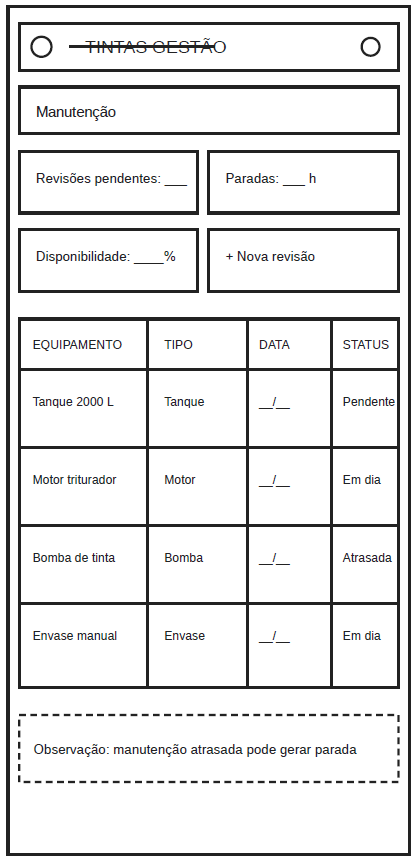
\includegraphics[width=0.45\textwidth]{figures/img3.png}
\caption{Wireframe Tela de Produção}
\label{fig:producao}
\end{figure}

\begin{figure}[h]
\centering
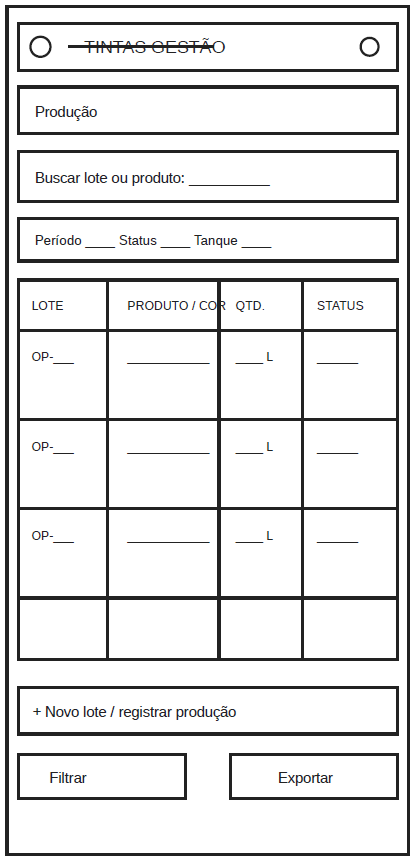
\includegraphics[width=0.45\textwidth]{figures/img4.png}
\caption{Wireframe Manutenção}
\label{fig:manutencao}
\end{figure}

\end{document}
